%%%%%%%%%%%%%%%%%%%%%%%%%%%%%%%%%%%%%%%%%%%%%%%%%%%%%%%%%%%%%%%%%%%
% CAPÍTULO 04: NAIVE BAYES
% AUTOR: Wilson Patricio Palma Samaniego
%%%%%%%%%%%%%%%%%%%%%%%%%%%%%%%%%%%%%%%%%%%%%%%%%%%%%%%%%%%%%%%%%%%

\setcounter{chapter}{3}
\chapter
  [Evaluación del algoritmo Naive Bayes]
  {Evaluación de la Efectividad del Algoritmo Naive Bayes en la Clasificación de Textos}
\label{cap:capitulo_04}

\textbf{Autor:} Wilson Patricio Palma Samaniego (wilson.palma@unl.edu.ec) \\
\textbf{Técnica asignada:} Naive Bayes \\

\section{Introducción}

En el contexto del libro, este capítulo se ubica dentro del eje temático \textit{Aprendizaje Estadístico y Modelos de Clasificación/Regresión}, con un enfoque técnico orientado a la evaluación de un clasificador probabilístico clásico. La pregunta que guía el desarrollo es concreta y delimitada: \textit{¿Qué tan efectivo es Naive Bayes en clasificación de texto?}. Esta cuestión resulta especialmente pertinente porque la clasificación textual constituye uno de los problemas más representativos de la minería de texto y del procesamiento de lenguaje natural, dos áreas donde la eficiencia computacional, la interpretabilidad y la robustez del modelo son tan importantes como su precisión predictiva.

Naive Bayes se ha mantenido como un algoritmo de referencia en tareas de clasificación supervisada por su simplicidad, su bajo costo computacional y su facilidad de implementación. Aun así, la literatura muestra que su desempeño no depende únicamente del algoritmo base, sino también de la representación de los datos, del balance de clases, del tamaño del corpus, del ruido léxico y de las técnicas de mejora que se incorporen al flujo de trabajo \cite{Kim2006,Frank2006,Kibriya2005,Schneider2005}. Por ello, más que preguntar si Naive Bayes \textit{sirve} o \textit{no sirve}, la pregunta técnicamente más útil es en qué condiciones su desempeño es competitivo y qué mecanismos permiten fortalecerlo \cite{Jiang2016,10.1145/2911451.2911547,Tang20161602}.

Desde una perspectiva histórica, Naive Bayes no es un modelo nuevo, pero sí un modelo que ha permanecido vigente por una razón importante: ofrece una línea base sólida, interpretabilidad directa y una relación muy favorable entre complejidad y rendimiento. A diferencia de otros clasificadores que requieren ajustes más costosos, Naive Bayes puede implementarse rápidamente y evaluarse sobre grandes volúmenes de texto, lo que lo hace especialmente útil en escenarios académicos y prácticos \cite{Kim2006,10.1007/978-3-540-30586-6_76,CHEN20095432}. Sin embargo, su aparente sencillez no debe llevar a subestimar sus limitaciones, ya que el modelo puede degradarse cuando las palabras están fuertemente correlacionadas, cuando existen clases desbalanceadas o cuando el corpus presenta alta variabilidad semántica \cite{Ganiz20111022,Frank2006,ELHINDI2020106652}.

Este capítulo analiza esa cuestión desde tres ángulos complementarios. Primero, desarrolla los fundamentos teóricos necesarios para comprender el funcionamiento del clasificador. Segundo, presenta la metodología de revisión y jerarquización de la evidencia bibliográfica utilizada para el proyecto. Tercero, sintetiza el análisis de la literatura y responde la pregunta de investigación a partir de los patrones observados en los estudios seleccionados. El objetivo no es solo describir el algoritmo, sino valorar su efectividad como solución técnica para clasificación textual en escenarios reales y académicos.

\begin{figure}[htbp]
\centering
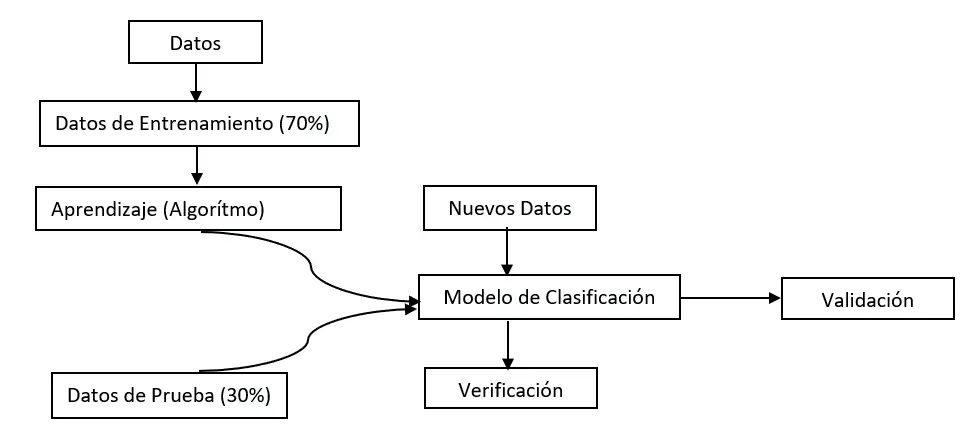
\includegraphics[width=0.9\textwidth]{figuras/esquema_evaluacion_naive_bayes.png}
\caption{Esquema conceptual de la evaluación de Naive Bayes en clasificación de textos.}
\label{fig:esquema_evaluacion}
\end{figure}

\subsection*{Alcance técnico del capítulo}

El alcance de este capítulo se centra en la clasificación textual como problema de aprendizaje supervisado. No se aborda la generación de texto, ni la traducción automática, ni la inferencia lingüística profunda; en cambio, se estudia Naive Bayes como clasificador probabilístico y como base metodológica para sistemas de minería de texto. El análisis se apoya en literatura que cubre tanto mejoras del algoritmo como aplicaciones concretas en análisis de sentimientos, clasificación documental, textos cortos, dominios especializados y problemas con datos escasos \cite{Sangounpao2019,Awotunde2023131,Pratmanto2020,Musleh2023,Wawer20191321,Humaidi2023,Mendoza2011251}.

\section{Fundamentos teóricos}

\subsection{Clasificación de textos y representación documental}

La clasificación de textos es una tarea de aprendizaje supervisado en la que un documento $d$ debe asignarse a una clase $c$ perteneciente a un conjunto finito $C$. En escenarios prácticos, el documento suele representarse mediante un vector de características derivado de su contenido léxico. La forma más común de representación es el modelo \textit{bag of words}, en el que el orden de las palabras se ignora y cada término aporta evidencia sobre la pertenencia del documento a una clase concreta.

Esta representación, aunque simplificada, es muy útil en clasificación textual porque convierte un problema de lenguaje natural en un problema numérico apto para modelos estadísticos. Sin embargo, también genera alta dimensionalidad, esparsidad y redundancia léxica. Por ello, la literatura sobre Naive Bayes en texto se ha concentrado en técnicas de selección y ponderación de características, así como en mecanismos para mejorar la estimación de probabilidades condicionales \cite{CHEN20095432,YOUN2009477,ZHANG2016137,Tang20162508,Ruan202020151}. La representación textual, por tanto, no es un detalle accesorio; es uno de los factores que más incide en la calidad final del clasificador.

Desde el punto de vista técnico, la clasificación textual suele enfrentar cuatro condiciones que afectan la precisión del modelo: vocabularios extensos, documentos muy breves, clases desbalanceadas y variabilidad semántica. Naive Bayes ofrece una respuesta atractiva a ese problema porque calcula probabilidades de pertenencia sin requerir procedimientos de optimización complejos. No obstante, su supuesto de independencia condicional entre atributos es una simplificación fuerte que puede limitar su rendimiento cuando los términos del documento presentan correlaciones semánticas o sintácticas significativas \cite{Ganiz20111022,Gan2021,Tang20161602}.

La literatura muestra que estas condiciones no son excepcionales, sino frecuentes en escenarios reales. En análisis de sentimientos, por ejemplo, los textos suelen ser cortos, ruidosos y altamente dependientes del contexto; en clasificación de documentos académicos, las categorías pueden estar desbalanceadas; y en dominios específicos, como medicina, contabilidad o sistemas de información, el vocabulario es muy especializado \cite{Sangounpao2019,Awotunde2023131,Pratmanto2020,Wang2007,Humaidi2023}. Por ello, el estudio de Naive Bayes no debe separarse de la estructura de los datos sobre los que opera.

\subsection{Teorema de Bayes y regla de decisión}

Naive Bayes se basa en el teorema de Bayes, una regla fundamental de la inferencia probabilística. Para una clase $c$ y un documento $d$, la probabilidad posterior se expresa como:

\begin{equation}
P(c \mid d) = \frac{P(c)\,P(d \mid c)}{P(d)}
\label{eq:bayes}
\end{equation}

En clasificación, el denominador $P(d)$ es constante para todas las clases, por lo que la decisión se toma maximizando el numerador. La regla de decisión se escribe como:

\begin{equation}
\hat{c} = \arg\max_{c \in C} P(c)\,P(d \mid c)
\label{eq:decision}
\end{equation}

Cuando el documento se representa como un conjunto de palabras $\{w_1, w_2, \dots, w_n\}$ y se asume independencia condicional entre ellas, el producto de probabilidades condicionales toma la forma:

\begin{equation}
\hat{c} = \arg\max_{c \in C} P(c)\prod_{i=1}^{n}P(w_i \mid c)
\label{eq:naive}
\end{equation}

La independencia condicional es la suposición que da nombre al algoritmo. En rigor, la suposición rara vez se cumple en lenguaje natural, pero el modelo sigue siendo útil porque la simplificación reduce drásticamente el número de parámetros a estimar y hace viable su aplicación en corpora grandes o medianos \cite{Kibriya2005,Frank2006,Schneider2005}. En otras palabras, Naive Bayes no busca modelar la estructura lingüística completa de un texto, sino capturar suficiente evidencia estadística para tomar decisiones útiles.

Para evitar problemas de subflujo numérico y facilitar el cálculo, la expresión anterior suele transformarse a escala logarítmica:

\begin{equation}
\hat{c} = \arg\max_{c \in C} \left[\log P(c) + \sum_{i=1}^{n}\log P(w_i \mid c)\right]
\label{eq:logdecision}
\end{equation}

Esta forma permite trabajar con sumas en lugar de productos y resulta más estable desde el punto de vista computacional. En clasificación de textos, la decisión final depende de la clase con mayor puntuación posterior, lo que convierte al algoritmo en un clasificador generativo de implementación directa. Aunque esta propiedad simplifica la inferencia, también explica por qué el clasificador es tan sensible a la calidad de la estimación probabilística y a la presencia de eventos raros o muy poco representados \cite{10.1007/978-3-540-71496-5_73,Frank2006,ELHINDI2020106652}.

\subsection{Modelo multinomial, suavizado y estimación de parámetros}

La variante más utilizada en clasificación textual es el modelo multinomial, en el que las frecuencias de las palabras dentro de cada clase se emplean para estimar probabilidades. Si $N_{w,c}$ representa el número de veces que la palabra $w$ aparece en documentos de la clase $c$, y $N_c$ el total de palabras observadas en esa clase, la estimación básica es:

\begin{equation}
P(w \mid c) = \frac{N_{w,c}}{N_c}
\label{eq:mnb_basic}
\end{equation}

El problema aparece cuando una palabra no se observa en el conjunto de entrenamiento para una clase específica, lo cual haría que la probabilidad condicional sea cero y anule completamente el producto de la ecuación \eqref{eq:naive}. Para resolverlo, se aplica suavizado, normalmente Laplace o alguna variante afín, de modo que:

\begin{equation}
P(w \mid c) = \frac{N_{w,c} + \alpha}{N_c + \alpha |V|}
\label{eq:smoothing}
\end{equation}

donde $|V|$ representa el tamaño del vocabulario y $\alpha$ es el parámetro de suavizado. Este mecanismo mejora la estabilidad de la estimación, especialmente cuando el corpus es pequeño o el vocabulario es muy amplio \cite{10.1007/978-3-540-71496-5_73}. En los estudios revisados, el suavizado aparece como una de las correcciones más sencillas y efectivas para hacer más robusto al clasificador. He y Ding muestran que incluso ligeras modificaciones en el proceso de suavizado pueden producir mejoras significativas en la clasificación \cite{10.1007/978-3-540-71496-5_73}.

La estimación de la probabilidad a priori $P(c)$ también es relevante, porque refleja la frecuencia relativa de cada clase en el conjunto de entrenamiento. Cuando existe desbalance, esta probabilidad puede sesgar fuertemente la predicción hacia las clases mayoritarias. Frank y Bouckaert muestran que ajustar los priors y corregir el tratamiento del desbalance mejora de manera importante el comportamiento de Naive Bayes en clasificación documental \cite{Frank2006}. En consecuencia, el rendimiento del algoritmo depende tanto del modelo de evidencia como de la calidad de las probabilidades previas.

Esta sensibilidad a la distribución de las clases también aparece en escenarios aplicados. Por ejemplo, la clasificación de sentimientos, la categorización de comentarios y la detección de tópicos en textos cortos suelen tener clases dominantes que distorsionan la frontera de decisión \cite{Pratmanto2020,Musleh2023,Risal202335,Wawer20191321}. En tales contextos, la corrección del desbalance deja de ser una mejora opcional y pasa a convertirse en un requisito metodológico para que el modelo sea realmente útil.

\subsection{Métricas para evaluar efectividad}

Hablar de efectividad en clasificación textual implica considerar varias dimensiones al mismo tiempo. Una sola métrica no basta para describir el comportamiento del modelo. En esta investigación, la efectividad se interpreta de forma integrada a partir de precisión, recall, F1 y costo computacional. En términos de clasificación binaria, las métricas básicas son:

\begin{equation}
\text{Precisión} = \frac{TP}{TP+FP}
\label{eq:precision}
\end{equation}

\begin{equation}
\text{Recall} = \frac{TP}{TP+FN}
\label{eq:recall}
\end{equation}

\begin{equation}
F1 = \frac{2 \cdot \text{Precisión} \cdot \text{Recall}}{\text{Precisión} + \text{Recall}}
\label{eq:f1}
\end{equation}

La precisión indica cuántas de las predicciones positivas fueron correctas; el recall mide cuántos positivos reales fueron recuperados; y el F1 resume ambos aspectos en una sola medida. Aunque en clasificación multiclase se utilizan variantes macro y micro, la lógica es la misma: una técnica es más efectiva si consigue equilibrio entre acierto, cobertura y estabilidad.

En la literatura sobre Naive Bayes, la comparación con otros clasificadores ha demostrado que el análisis debe ser más amplio que la simple exactitud global. Zhang et al. proponen una comparación bayesiana de clasificadores de texto para evitar las limitaciones de las pruebas frecuentistas tradicionales y capturar de forma más realista la incertidumbre de los resultados \cite{10.1145/2911451.2911547}. Esto es importante porque la \textit{efectividad} de un clasificador no se reduce a un número aislado; también incluye robustez, interpretabilidad, costo de entrenamiento y sensibilidad al contexto.

Tang et al. señalan además que, en clasificación textual, el rendimiento de Naive Bayes no debe evaluarse únicamente en función de su exactitud, sino también de su comportamiento frente a diferentes representaciones de rasgos y configuraciones de selección de atributos \cite{Tang20162508}. De este modo, la evaluación se vuelve multidimensional y más cercana a las condiciones reales de uso.

\subsection{Variantes y mejoras del algoritmo}

El análisis de la literatura muestra que el Naive Bayes clásico suele mejorarse mediante cuatro líneas técnicas principales: selección de características, ponderación de atributos, relajación del supuesto de independencia y adaptación al dominio semántico o al cambio de distribución.

La primera línea de mejora es la selección de características. En textos, el vocabulario suele ser muy amplio y gran parte de los términos aporta poca discriminación. Chen et al. proponen métricas específicas de evaluación de rasgos para Naive Bayes, mientras que Youn y Jeong introducen un esquema de \textit{class dependent feature scaling} que incrementa la capacidad de discriminación del modelo \cite{CHEN20095432,YOUN2009477}. De modo semejante, Tang, Kay y He muestran que la selección óptima de características puede mejorar significativamente la clasificación con Naive Bayes sin sacrificar su simplicidad \cite{Tang20162508,Tang20161602}. En el mismo eje, Feng et al. proponen una selección de subconjuntos de características que resulta competitiva frente a otros esquemas de ponderación y modelos de referencia \cite{FENG2015109}.

La segunda línea es la ponderación de características. Kim et al. muestran que la normalización por documento y el \textit{feature weighting} permiten que Naive Bayes compita con métodos más complejos en clasificación textual \cite{Kim2006}. Jiang et al. van más allá al proponer una ponderación profunda de características que mejora el modelo base en múltiples conjuntos de datos \cite{Jiang2016}. En una dirección similar, Zhang et al. presentan dos enfoques de ponderación que mantienen el bajo costo computacional y elevan la precisión \cite{ZHANG2016137}. Estas propuestas son especialmente relevantes porque resuelven una debilidad conocida del modelo: su tratamiento uniforme de las palabras dentro de una clase. Ruan et al. amplían esta línea con ponderación profunda específica por clase, mostrando que el ajuste fino de pesos sigue siendo un camino efectivo para mejorar el comportamiento del modelo \cite{Ruan202020151}.

La tercera línea es la relajación del supuesto de independencia condicional. Ganiz et al. proponen un Naive Bayes de orden superior, no IID, capaz de capturar dependencias que el modelo clásico ignora \cite{Ganiz20111022}. Ding et al. desarrollan un clasificador bayesiano novedoso que busca relajaciones funcionales de ese supuesto \cite{4554061}. Más recientemente, Gan et al. adaptan \textit{hidden naive Bayes} para texto, y El Hindi et al. proponen algoritmos de \textit{lazy fine-tuning} para mejorar el desempeño en clasificación textual \cite{Gan2021,ELHINDI2020106652}. Estos trabajos muestran que el modelo sigue evolucionando sin perder su esencia probabilística.

La cuarta línea es la adaptación al dominio semántico o al cambio de distribución. Kim et al. integran información basada en Wikipedia para construir un Naive Bayes semántico con alta efectividad en corpora de referencia \cite{KIM2018128}. En otro contexto, Dai et al. desarrollan un enfoque de transferencia de conocimiento entre dominios con Naive Bayes para cuando los datos de entrenamiento y prueba no siguen la misma distribución \cite{10.5555/1619645.1619732}. Ambas propuestas confirman que Naive Bayes no es un algoritmo estático; puede ampliarse para responder mejor a condiciones complejas y heterogéneas.

Una quinta línea, que también aparece en la literatura, es la hibridación con otras estrategias de clasificación o con técnicas de aprendizaje local. Lu et al. combinan Naive Bayes con un clasificador asociativo para mejorar el tratamiento de textos en chino \cite{LU2010598}. A nivel más general, Awotunde et al. presentan un sistema de reseñas hoteleras basado en un ensamble donde Naive Bayes participa como componente de decisión \cite{Awotunde2023131}. Estas aproximaciones muestran que el valor del algoritmo no siempre radica en ser el clasificador final, sino en funcionar como núcleo estadístico dentro de soluciones más amplias.

La tabla siguiente resume, desde una perspectiva técnica, las principales dimensiones que aparecen reiteradamente en la literatura revisada.

\begin{table}[htbp]
\centering
\caption{Dimensiones técnicas de la efectividad de Naive Bayes en clasificación de textos}
\label{tab:dimensiones}
\begin{tabular}{|p{3.2cm}|p{6.0cm}|p{5.3cm}|}
\hline
\textbf{Dimensión} & \textbf{Hallazgo recurrente en la literatura} & \textbf{Implicación técnica} \\
\hline
Precisión & Mejora cuando se combinan selección y ponderación de características \cite{Kim2006,Jiang2016,ZHANG2016137,FENG2015109}. & Aumenta la capacidad discriminativa del modelo. \\
\hline
Robustez & Funciona bien en textos cortos, corpus pequeños y dominios específicos \cite{Sangounpao2019,Awotunde2023131,Pratmanto2020,Wawer20191321}. & Es útil en escenarios reales con datos limitados. \\
\hline
Adaptabilidad & Variantes como higher-order NB, hidden NB y semantic NB extienden el modelo base \cite{Ganiz20111022,Gan2021,KIM2018128}. & El algoritmo puede adaptarse a contextos más complejos. \\
\hline
Estabilidad & El suavizado y el ajuste de priors reducen errores de estimación \cite{Frank2006,10.1007/978-3-540-71496-5_73}. & Evita probabilidades nulas y sesgo por clases. \\
\hline
Interpretabilidad & Su formulación probabilística es clara y directa \cite{Kim2006,Frank2006}. & Facilita su explicación y uso académico. \\
\hline
Costo computacional & Mantiene baja complejidad de entrenamiento y predicción \cite{Jiang2016,CHEN20095432}. & Es viable para sistemas con recursos limitados. \\
\hline
Generalización & El desempeño cae si el dominio cambia demasiado o si la distribución de datos es distinta \cite{10.5555/1619645.1619732,ELHINDI2020106652}. & Obliga a aplicar transferencia o ajuste local. \\
\hline
\end{tabular}
\end{table}

\begin{figure}[htbp]
\centering
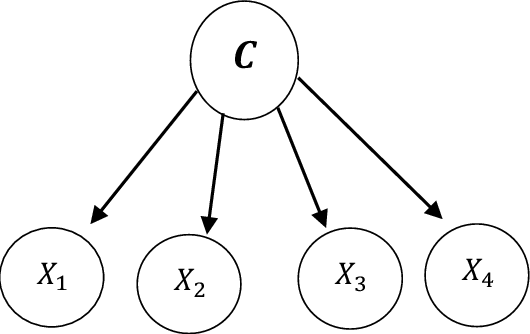
\includegraphics[width=0.92\textwidth]{figuras/estructura_conceptual_naive_bayes.png}
\caption{Estructura conceptual del clasificador Naive Bayes aplicado a documentos de texto.}
\label{fig:estructura_nb}
\end{figure}

\section{Metodología y análisis de la literatura}

\subsection{Estrategia metodológica general}

La metodología seguida para este capítulo se apoyó en la lógica general de trabajo usada durante toda la asignatura. Primero, la pregunta de investigación se descompuso en palabras clave principales y términos asociados. Después, se construyeron cadenas de búsqueda con operadores lógicos para recuperar estudios en bases como IEEE Xplore y ACM Digital Library. El primer corte produjo una matriz inicial de cinco artículos científicos, lo que permitió empezar la extracción y la lectura analítica de manera controlada.

Posteriormente, la búsqueda se amplió a fuentes como ScienceDirect, Springer y Lens para reunir un corpus de veinte referencias sólidas y luego, en una fase de mayor refinamiento, se utilizó Scopus para obtener metadatos y consolidar una base de cuarenta y cuatro artículos relacionados con la pregunta de investigación. En ese proceso se usaron Mendeley o Zotero para la gestión bibliográfica, Overleaf para la escritura en LaTeX y NotebookLM para jerarquizar y organizar la información extraída. Esta secuencia metodológica no solo permitió localizar literatura, sino también clasificarla, compararla y convertirla en evidencia argumentativa para responder la pregunta planteada.

Además, la metodología general proporcionada por el docente enfatiza una lógica progresiva: definición de cadenas de búsqueda, ejecución en bases especializadas, construcción de matrices iniciales, ampliación del corpus, jerarquización mediante herramientas de apoyo y exportación de metadatos en BibTeX. Esa secuencia se refleja con claridad en el trabajo realizado en este proyecto y explica por qué la revisión no se limita a un conjunto pequeño de artículos, sino que culmina en una base documental amplia y trazable. En términos metodológicos, esto es importante porque demuestra que la revisión no es improvisada, sino sistemática y reproducible \cite{10.1145/2911451.2911547,Tang20161602,Awotunde2023131}.

\begin{figure}[htbp]
\centering
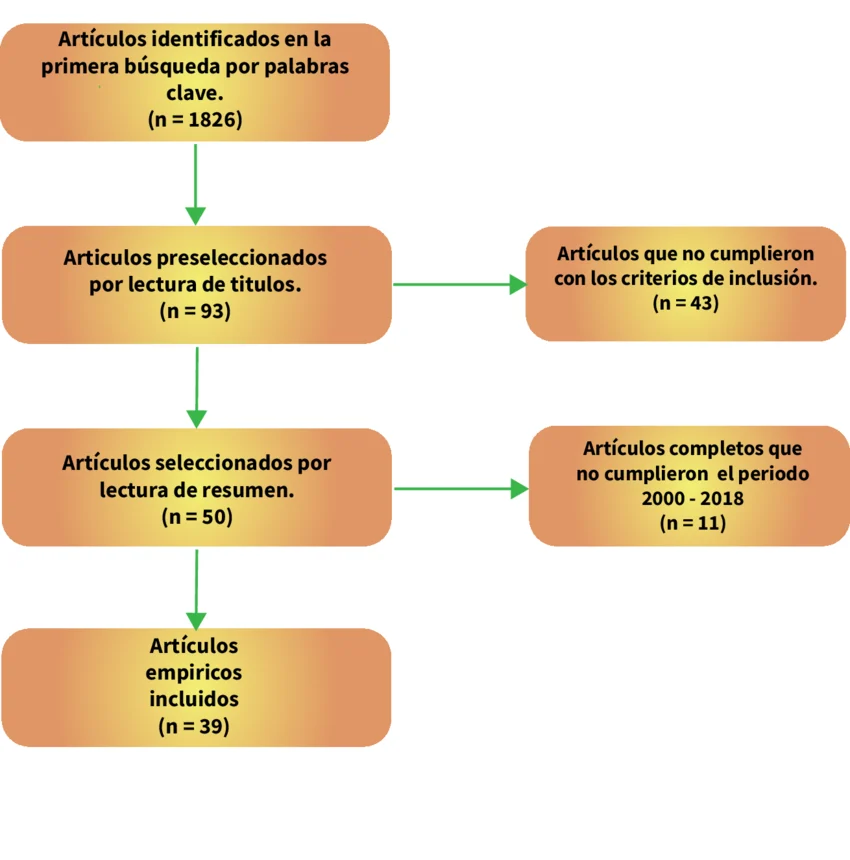
\includegraphics[width=0.9\textwidth]{figuras/flujo_metodologico_general.png}
\caption{Flujo metodológico general seguido para la búsqueda, selección y análisis de la literatura.}
\label{fig:flujo_metodologico}
\end{figure}

La lógica de selección de la literatura se basó en dos criterios centrales: relevancia temática y aporte técnico. La relevancia temática se definió por la relación directa del artículo con Naive Bayes y clasificación textual; el aporte técnico, por su capacidad para explicar, mejorar o comparar el comportamiento del algoritmo. Bajo esa lógica, los trabajos que estudian técnicas de selección de rasgos, ponderación, suavizado, adaptación semántica o relajación del supuesto de independencia fueron considerados más útiles que aquellos centrados únicamente en aplicaciones muy específicas sin discusión metodológica profunda.

\begin{table}[htbp]
\centering
\caption{Criterios de inclusión y exclusión empleados en el análisis bibliográfico}
\label{tab:criterios}
\begin{tabular}{|p{3.2cm}|p{5.8cm}|p{5.5cm}|}
\hline
\textbf{Criterio} & \textbf{Inclusión} & \textbf{Exclusión} \\
\hline
Relación con el tema & Estudios centrados en Naive Bayes, clasificación de texto o variantes del modelo. & Trabajos sin vínculo directo con clasificación textual o sin referencia al algoritmo. \\
\hline
Aporte técnico & Artículos que mejoran, comparan o adaptan el clasificador. & Estudios meramente descriptivos sin aporte metodológico claro. \\
\hline
Tipo de evidencia & Experimentos, métricas de clasificación, análisis comparativo, validación cruzada. & Opiniones no justificadas o textos sin metodología explícita. \\
\hline
Utilidad para la pregunta & Fuentes que ayudan a responder qué tan efectivo es Naive Bayes en texto. & Fuentes que no permiten extraer conclusiones sobre desempeño. \\
\hline
\end{tabular}
\end{table}

\subsection{Estructura de la evidencia recuperada}

La revisión bibliográfica mostró una evolución ordenada en varias etapas: búsqueda inicial de cinco artículos, análisis de brechas, clasificación de enfoques, mapa conceptual, formulación de objetivos, ampliación a veinte fuentes y, finalmente, recuperación de cuarenta y cuatro artículos con metadatos completos. Esta secuencia es importante porque demuestra trazabilidad y madurez progresiva del proyecto. No se trató de acumular referencias de manera indiscriminada, sino de construir un corpus cada vez más preciso y útil.

\begin{table}[htbp]
\centering
\caption{Síntesis de las etapas de construcción del corpus bibliográfico}
\label{tab:etapas}
\begin{tabular}{|p{2.4cm}|p{2.8cm}|p{8.0cm}|}
\hline
\textbf{Etapa} & \textbf{Producto} & \textbf{Propósito} \\
\hline
APE2 & Matriz de cinco artículos & Obtener evidencia preliminar sobre la efectividad del algoritmo. \\
\hline
APE3 & Análisis de brechas & Identificar limitaciones, vacíos y problemas recurrentes. \\
\hline
ACD3 & Tabla de enfoques & Verificar el tipo de investigación predominante en la literatura. \\
\hline
AA3 & Mapa conceptual & Delimitar problema, contexto, actores y objetivos. \\
\hline
APE4 & Pregunta y objetivos & Traducir la brecha en una ruta de investigación clara. \\
\hline
APE5 & Veinte fuentes & Consolidar antecedentes y ampliar el estado del arte. \\
\hline
APE6 & Cuarenta y cuatro artículos y BibTeX & Organizar la base documental final para el análisis técnico. \\
\hline
AA6 & Antecedentes iniciales & Sintetizar la evidencia en una narrativa académica coherente. \\
\hline
\end{tabular}
\end{table}

\subsection{Análisis temático de la literatura}

Al analizar las cuarenta y cuatro fuentes reunidas, la evidencia se agrupa en cinco grandes ejes: mejoras al modelo base, selección y ponderación de características, variantes no IID o de orden superior, adaptación semántica o por transferencia, y aplicaciones en dominios específicos. Esa organización permite ver que la efectividad de Naive Bayes no es uniforme, sino dependiente del tipo de problema textual.

\paragraph{1. Mejoras al modelo base}

Los estudios más tempranos muestran que el Naive Bayes multinomial puede mejorar notablemente si se corrigen sus problemas de estimación. Kim et al. proponen normalización por documento y ponderación de características, obteniendo resultados comparables a clasificadores más complejos \cite{Kim2006}. De forma similar, Kibriya et al. revisan el desempeño del modelo multinomial y señalan que TF-IDF y la normalización son componentes importantes para elevar su rendimiento \cite{Kibriya2005}. En esta misma línea, Schneider enfatiza que el bajo desempeño de Naive Bayes no se debe a una falla total del método, sino a una modelación incompleta del texto y a una selección inadecuada de atributos \cite{10.1007/978-3-540-30586-6_76}.

A este grupo se suman los trabajos que mejoran el modelo mediante ajustes prácticos y refinamientos de la estimación. He y Ding muestran que el suavizado puede estabilizar el comportamiento del clasificador, especialmente cuando el vocabulario es amplio y los ejemplos etiquetados son escasos \cite{10.1007/978-3-540-71496-5_73}. De manera complementaria, Narayanan et al. presentan un modelo mejorado para análisis de sentimientos, resaltando que pequeños cambios en la representación y en la estimación pueden generar mejoras notables en el rendimiento \cite{Narayanan2013194}. En ambos casos, el mensaje técnico es claro: Naive Bayes no debe ser juzgado solo por su versión más simple, sino por las posibilidades de ajuste que admite.

\paragraph{2. Selección y ponderación de características}

La literatura es consistente al señalar que la selección de rasgos es uno de los factores más importantes para la efectividad del algoritmo. Chen et al. proponen medidas específicas para seleccionar características relevantes en textos multiclase \cite{CHEN20095432}. Youn y Jeong presentan una técnica de escalado dependiente de la clase que mejora la capacidad del clasificador para distinguir entre categorías \cite{YOUN2009477}. Tang, Kay y He muestran, además, que acercarse a una selección óptima puede traducirse en mejoras sustanciales de desempeño sin comprometer la simplicidad del modelo \cite{Tang20162508,Tang20161602}. A esto se suman Jiang et al., quienes incorporan \textit{deep feature weighting}, y Zhang et al., que diseñan dos estrategias de ponderación con beneficios concretos en precisión \cite{Jiang2016,ZHANG2016137}. Feng et al. agregan otra perspectiva al plantear la selección de subconjuntos de características, lo que confirma la centralidad de esta línea de trabajo \cite{FENG2015109}.

Desde un punto de vista interpretativo, estos estudios indican que la principal debilidad de Naive Bayes en texto no está en el teorema de Bayes, sino en la representación de los atributos. Si los atributos están mal elegidos, poco informativos o excesivamente redundantes, la capacidad discriminativa del modelo se reduce. Si, por el contrario, se seleccionan y ponderan adecuadamente, el clasificador puede recuperar una gran parte de su efectividad, incluso en escenarios complejos \cite{Kim2006,Jiang2016,ZHANG2016137,Tang20162508}.

\paragraph{3. Variantes no IID y modelos extendidos}

Una de las limitaciones más conocidas del modelo clásico es su supuesto de independencia condicional. Cuando las palabras están correlacionadas, la hipótesis naive se vuelve demasiado restrictiva. Ganiz et al. responden a este problema proponiendo un Naive Bayes de orden superior que modela dependencias entre atributos \cite{Ganiz20111022}. Ding et al. también presentan un clasificador bayesiano novedoso que busca relajaciones funcionales de ese supuesto \cite{4554061}. Más recientemente, Gan et al. adaptan \textit{hidden naive Bayes} para texto y El Hindi et al. proponen un mecanismo de \textit{lazy fine-tuning} para mejorar el desempeño local del modelo \cite{Gan2021,ELHINDI2020106652}. Estos trabajos demuestran que Naive Bayes sigue siendo una plataforma fértil para el desarrollo de variantes técnicas.

La importancia de estas variantes no es únicamente académica. En clasificación de texto, las palabras suelen aparecer en grupos semánticamente relacionados, y muchas veces el significado de un documento depende de combinaciones de términos más que de términos aislados. Por ello, los modelos que intentan capturar dependencias o relaciones de contexto tienden a mejorar el comportamiento del clasificador. El resultado no es necesariamente una sustitución del modelo base, sino una extensión de su capacidad de representación \cite{Ganiz20111022,Gan2021,ELHINDI2020106652}.

\paragraph{4. Adaptación semántica y transferencia entre dominios}

Otra línea de evolución importante consiste en incorporar información semántica o de dominio. Kim et al. utilizan conceptos asociados a Wikipedia para enriquecer la representación documental y mejorar el clasificador \cite{KIM2018128}. En otro contexto, Dai et al. desarrollan un enfoque de transferencia de conocimiento entre dominios con Naive Bayes para cuando los datos de entrenamiento y prueba no siguen la misma distribución \cite{10.5555/1619645.1619732}. Ambas propuestas confirman que Naive Bayes no es un algoritmo estático; puede ampliarse para responder mejor a condiciones complejas y heterogéneas.

Este punto es crucial porque muchos problemas de clasificación textual reales no ocurren en un entorno limpio y homogéneo. Los textos cambian de estilo, de idioma, de dominio y de estructura. En esos casos, la adaptación semántica o la transferencia entre dominios permiten que el modelo siga siendo útil sin requerir un rediseño completo. Desde la óptica de efectividad, esto significa que el algoritmo puede mantener un desempeño razonable incluso cuando el problema no coincide exactamente con el corpus de entrenamiento \cite{KIM2018128,10.5555/1619645.1619732,Wang2007}.

\paragraph{5. Aplicaciones en dominios específicos}

La efectividad de Naive Bayes también se verifica en tareas concretas. Sangounpao y Muenchaisri lo aplican a texto corto en un conjunto de datos pequeño, con apoyo ontológico \cite{Sangounpao2019}. Awotunde et al. lo integran en un sistema de análisis de reseñas de hoteles \cite{Awotunde2023131}. Pratmanto et al. lo usan en análisis de opiniones sobre aplicaciones móviles y Musleh et al. lo aplican al análisis de comentarios en YouTube \cite{Pratmanto2020,Musleh2023}. También se reportan usos en textos cortos en polaco, clasificación académica y categorización documental \cite{Wawer20191321,Humaidi2023,Wang2007,Mendoza2011251}. Estos estudios no siempre buscan perfeccionar el algoritmo, pero sí demuestran que su desempeño práctico sigue siendo útil en contextos variados.

La relevancia de estas aplicaciones está en que permiten observar el comportamiento del clasificador fuera del laboratorio. A veces, Naive Bayes no supera a los métodos más complejos en precisión pura, pero sí ofrece una relación más favorable entre rendimiento, rapidez y facilidad de integración. En aplicaciones reales, esa relación puede ser más valiosa que una pequeña mejora porcentual en exactitud \cite{Awotunde2023131,Pratmanto2020,Musleh2023,Risal202335,Wawer20191321}. Además, la existencia de estudios en dominios tan diversos como biomedicina, análisis de sentimientos, sistemas académicos y categorización documental confirma que la técnica conserva versatilidad \cite{Han20062136,Wang2007,Mendoza2011251}.

\begin{table}[htbp]
\centering
\caption{Estrategias de mejora de Naive Bayes y su efecto observado en la literatura}
\label{tab:mejoras}
\begin{tabular}{|p{4.1cm}|p{3.4cm}|p{4.0cm}|p{4.0cm}|}
\hline
\textbf{Estrategia} & \textbf{Referencias representativas} & \textbf{Efecto principal} & \textbf{Observación técnica} \\
\hline
Normalización y ponderación por documento & \cite{Kim2006,Kibriya2005} & Mejora la calidad de la estimación de probabilidades. & Permite competir con clasificadores más complejos. \\
\hline
Selección de características & \cite{CHEN20095432,YOUN2009477,Tang20162508,FENG2015109} & Reduce ruido y esparsidad del vocabulario. & Incrementa discriminación y estabilidad. \\
\hline
Ponderación de características & \cite{Jiang2016,ZHANG2016137,Ruan202020151} & Ajusta el peso de términos relevantes por clase. & Eleva la precisión sin perder simplicidad. \\
\hline
Suavizado y ajuste de priors & \cite{Frank2006,10.1007/978-3-540-71496-5_73} & Evita probabilidades nulas y sesgo por clases desbalanceadas. & Mejora robustez y estabilidad numérica. \\
\hline
Modelos no IID o de orden superior & \cite{Ganiz20111022,4554061,Gan2021} & Captura dependencias entre términos. & Reduce la rigidez del supuesto naive. \\
\hline
Adaptación semántica o por transferencia & \cite{KIM2018128,10.5555/1619645.1619732} & Mejora rendimiento en dominios cambiantes o enriquecidos semánticamente. & Amplía la aplicabilidad del modelo. \\
\hline
Ajuste local y fine-tuning & \cite{ELHINDI2020106652} & Recalibra probabilidades según vecinos cercanos o contexto local. & Es útil cuando el conjunto de entrenamiento es limitado. \\
\hline
Hibridación con otros enfoques & \cite{LU2010598,Awotunde2023131} & Combina fortalezas de distintos clasificadores. & Puede mejorar la exactitud sin perder simplicidad básica. \\
\hline
\end{tabular}
\end{table}

\subsection{Síntesis del análisis de la literatura}

El análisis integrado de la evidencia permite formular una conclusión intermedia muy clara: Naive Bayes es técnicamente efectivo para clasificación textual, pero su rendimiento depende del tratamiento previo del texto y del tipo de mejora aplicada al modelo. En su forma básica puede quedar por debajo de métodos más sofisticados en algunos conjuntos de datos, pero con selección de características, ponderación, suavizado y ajustes estructurales, su comportamiento mejora de manera consistente \cite{Kim2006,Frank2006,Jiang2016,ZHANG2016137,Tang20162508,FENG2015109}.

La literatura también sugiere que la comparación entre clasificadores no debe hacerse únicamente con la idea de \textit{ganador absoluto}. Zhang et al. muestran que la comparación bayesiana ofrece una visión más completa que las pruebas tradicionales \cite{10.1145/2911451.2911547}. Ese enfoque es importante porque, en clasificación textual, el mejor clasificador no siempre es el más complejo, sino el que mejor se adapta al corpus, a la métrica y a las restricciones de uso. En ese sentido, Naive Bayes conserva ventaja en escenarios donde se valora rapidez, interpretabilidad y capacidad suficiente con recursos limitados.

La evidencia revisada también permite observar un patrón transversal: cuando el texto es corto, el vocabulario es escaso, o la clase está desbalanceada, el Naive Bayes básico puede fallar si no se aplican ajustes adicionales \cite{Sangounpao2019,Frank2006,Pratmanto2020,Wawer20191321}. En cambio, cuando se introducen técnicas de ponderación, selección de rasgos, suavizado o adaptación semántica, el clasificador logra una respuesta mucho más estable y, en varios casos, competitiva frente a alternativas más complejas \cite{Kim2006,Jiang2016,Gan2021,KIM2018128}.

\begin{figure}[htbp]
\centering
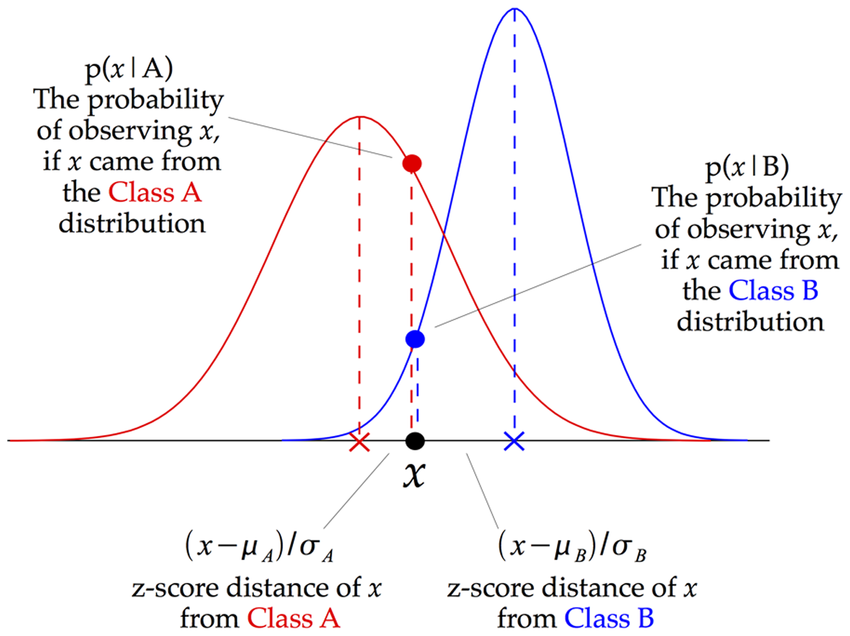
\includegraphics[width=0.9\textwidth]{figuras/relacion_mejoras_naive_bayes.png}
\caption{Relación entre las principales técnicas de mejora y el incremento observado en la efectividad de Naive Bayes.}
\label{fig:relacion_mejoras}
\end{figure}

\subsection{Discusión técnica de los resultados}

Desde una perspectiva de ingeniería, la principal fortaleza de Naive Bayes radica en que permite construir soluciones rápidas y explicables. Su principal debilidad es que simplifica demasiado la estructura del texto. Esa tensión entre simplicidad y exactitud es precisamente la que explica por qué el algoritmo sigue vigente: cuando el costo computacional, la facilidad de implementación y la interpretabilidad son prioritarios, Naive Bayes resulta muy atractivo; cuando la dependencia entre atributos es fuerte y el corpus es complejo, entonces requiere ajustes para no perder competitividad \cite{Schneider2005,Ganiz20111022,Tang20161602}.

Además, la literatura muestra que su utilidad no es homogénea en todos los dominios. En análisis de sentimientos y reseñas, los textos suelen ser breves pero abundantes, lo que favorece modelos rápidos y robustos \cite{Pratmanto2020,Musleh2023,Risal202335}. En clasificación académica o documental, la estructura del lenguaje puede ser más formal, pero también más desbalanceada, lo que hace relevantes los ajustes de priors \cite{Frank2006,Wang2007,Mendoza2011251}. En contextos especializados, como biomedicina o sistemas de información, la selección de características se vuelve esencial \cite{Han20062136,Humaidi2023}. En todos los casos, Naive Bayes conserva valor práctico, pero su desempeño depende de decisiones de modelado concretas.

Otro punto clave es que Naive Bayes funciona como una excelente línea base. Incluso cuando no es la mejor técnica final, su rendimiento ofrece una referencia confiable para comparar métodos más elaborados. Este papel de \textit{baseline} es importante en investigación porque permite medir si una mejora realmente aporta valor. En ese sentido, el modelo no solo sirve como solución final, sino como instrumento metodológico para la evaluación comparativa \cite{10.1145/2911451.2911547,Tang20162508,ELHINDI2020106652}.

\section{Conclusiones}

La pregunta de investigación planteada en este capítulo puede responderse con base en la evidencia revisada: Naive Bayes es una técnica efectiva para clasificación de texto, pero su efectividad es condicional y no absoluta. Su desempeño es especialmente sólido cuando el problema presenta alta dimensionalidad, textos breves, necesidad de interpretación rápida y restricciones de costo computacional. En esos escenarios, el clasificador mantiene una relación favorable entre simplicidad y rendimiento \cite{Kim2006,Frank2006,Sangounpao2019,Awotunde2023131,Pratmanto2020}.

Sin embargo, la efectividad del modelo mejora de forma notoria cuando se aplican técnicas complementarias. La selección de características reduce ruido y esparsidad; la ponderación de atributos incrementa la discriminación entre clases; el suavizado corrige probabilidades nulas; y las variantes no IID, semánticas o de ajuste local compensan las limitaciones del supuesto de independencia condicional \cite{CHEN20095432,YOUN2009477,Jiang2016,ZHANG2016137,FENG2015109,Ganiz20111022,Gan2021,ELHINDI2020106652}. Por tanto, el Naive Bayes clásico debe entenderse como una base metodológica robusta, pero no necesariamente como su forma final más potente.

También se concluye que la comparación justa de Naive Bayes con otros clasificadores exige una evaluación rigurosa. En algunos corpora, variantes mejoradas del modelo pueden acercarse a la precisión de clasificadores más complejos e incluso competir de forma equilibrada con ellos \cite{Kim2006,10.1145/2911451.2911547,KIM2018128}. Esto confirma que la simplicidad no implica necesariamente bajo rendimiento; más bien, obliga a analizar cuidadosamente el tipo de problema, la calidad de las características y la estrategia de modelado empleada.

Finalmente, el capítulo permite afirmar que Naive Bayes sigue siendo una técnica vigente, útil y teóricamente sólida para la clasificación de textos. No es el clasificador universalmente mejor, pero sí uno de los más versátiles y didácticos para construir soluciones de minería textual cuando se combina con técnicas de mejora apropiadas. Desde el punto de vista técnico, su efectividad no radica únicamente en la fórmula bayesiana, sino en la manera en que se adapta a la estructura real del lenguaje y a las condiciones del corpus.